\begin{figure}[H]
  \centering
    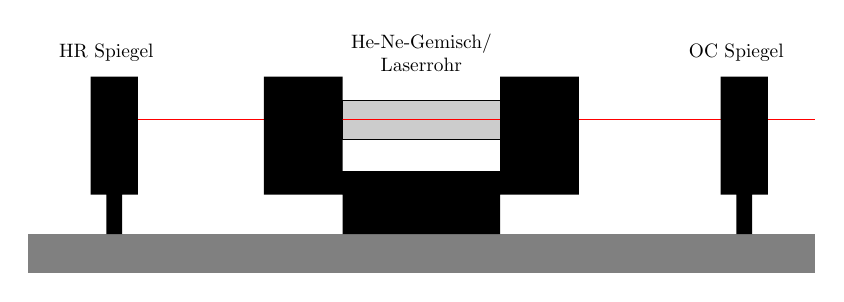
\begin{tikzpicture}
    \fill[white!50!black] (0,0)--(10,0)--(10,0.5)--(0,0.5)--cycle;
    \filldraw[fill=black!20!white] (4,2.2)--(6,2.2)--(6,1.7)--(4,1.7)--cycle;
    \node[scale=0.7,align=center] at (5,2.8) {He-Ne-Gemisch/\\Laserrohr};
    \draw[red] (1,1.95)--(10,1.95);

    \fill (1,0.5)--(1,1)--(0.8,1)--(0.8,2.5)--(1.4,2.5)--(1.4,1)--(1.2,1)--(1.2,0.5)--cycle;
    \node[scale=0.7] at (1,2.8) {HR Spiegel};
    \fill (9,0.5)--(9,1)--(8.8,1)--(8.8,2.5)--(9.4,2.5)--(9.4,1)--(9.2,1)--(9.2,0.5)--cycle;
    \node[scale=0.7] at (9,2.8) {OC Spiegel};

    \fill (4,0.5)--(4,1)--(3,1)--(3,2.5)--(4,2.5)--(4,1.3)--(6,1.3)--(6,2.5)--(7,2.5)--(7,1)--(6,1)--(6,0.5)--cycle;
    \end{tikzpicture}
  \caption{Skizze des Versuchsaufbaus}
  \label{fig:aufbau}
\end{figure}
